%%
%% Copyright 2007, 2008, 2009 Elsevier Ltd
%%
%% This file is part of the 'Elsarticle Bundle'.
%% ---------------------------------------------
%%
%% It may be distributed under the conditions of the LaTeX Project Public
%% License, either version 1.2 of this license or (at your option) any
%% later version.  The latest version of this license is in
%%    http://www.latex-project.org/lppl.txt
%% and version 1.2 or later is part of all distributions of LaTeX
%% version 1999/12/01 or later.
%%
%% The list of all files belonging to the 'Elsarticle Bundle' is
%% given in the file `manifest.txt'.
%%

%% Template article for Elsevier's document class `elsarticle'
%% with harvard style bibliographic references
%% SP 2008/03/01
%%
%%
%%
%% $Id: elsarticle-template-harv.tex 4 2009-10-24 08:22:58Z rishi $
%%
%%
%% \documentclass[preprint,authoryear,12pt]{elsarticle}

%% Use the option review to obtain double line spacing
%% \documentclass[authoryear,preprint,review,12pt]{elsarticle}

%% Use the options 1p,twocolumn; 3p; 3p,twocolumn; 5p; or 5p,twocolumn
%% for a journal layout:
%% \documentclass[final,authoryear,1p,times]{elsarticle}
%% \documentclass[final,authoryear,1p,times,twocolumn]{elsarticle}
%% \documentclass[final,authoryear,3p,times]{elsarticle}
\documentclass[final,authoryear,3p,times,twocolumn]{elsarticle}
%% \documentclass[final,authoryear,5p,times]{elsarticle}
%% \documentclass[final,authoryear,5p,times,twocolumn]{elsarticle}
%%-------------------------------------------------------------------------------
%add ukrainian locale
\usepackage[ukrainian,russian,english]{babel}
\usepackage[utf8]{inputenc}
\usepackage[T2A]{fontenc}
%mathematical symbols
\usepackage{gensymb}
%%-------------------------------------------------------------------------------


%% if you use PostScript figures in your article
%% use the graphics package for simple commands
%% \usepackage{graphics}
%% or use the graphicx package for more complicated commands
\usepackage{graphicx}
%% or use the epsfig package if you prefer to use the old commands
\usepackage{epsfig}

%% The amssymb package provides various useful mathematical symbols
\usepackage{amssymb}
%% The amsthm package provides extended theorem environments
%% \usepackage{amsthm}

%% The lineno packages adds line numbers. Start line numbering with
%% \begin{linenumbers}, end it with \end{linenumbers}. Or switch it on
%% for the whole article with \linenumbers after \end{frontmatter}.
%% \usepackage{lineno}

%% for sub[super]script
\usepackage{fixltx2e}

%% natbib.sty is loaded by default. However, natbib options can be
%% provided with \biboptions{...} command. Following options are
%% valid:

%%   round  -  round parentheses are used (default)
%%   square -  square brackets are used   [option]
%%   curly  -  curly braces are used      {option}
%%   angle  -  angle brackets are used    <option>
%%   semicolon  -  multiple citations separated by semi-colon (default)
%%   colon  - same as semicolon, an earlier confusion
%%   comma  -  separated by comma
%%   authoryear - selects author-year citations (default)
%%   numbers-  selects numerical citations
%%   super  -  numerical citations as superscripts
%%   sort   -  sorts multiple citations according to order in ref. list
%%   sort&compress   -  like sort, but also compresses numerical citations
%%   compress - compresses without sorting
%%   longnamesfirst  -  makes first citation full author list
%%
\bibliographystyle{ieeetr}
\biboptions{numbers,square}

%% \biboptions{}

\journal{Physica B}

\begin{document}

\begin{frontmatter}

%% Title, authors and addresses

%% use the tnoteref command within \title for footnotes;
%% use the tnotetext command for the associated footnote;
%% use the fnref command within \author or \address for footnotes;
%% use the fntext command for the associated footnote;
%% use the corref command within \author for corresponding author footnotes;
%% use the cortext command for the associated footnote;
%% use the ead command for the email address,
%% and the form \ead[url] for the home page:
%%

\title{{\LARGE An EPR studies of V\textsubscript{C}C\textsubscript{Si}\textsuperscript{-} defect in neutron irradiated 3C-SiC}}
%% \tnotetext[label1]{}
\author[dep]{V. Bratus'\corref{cor1}}
\ead{v\_bratus@isp.kiev.ua}

\author[dep]{R. Melnyk\corref{cor2}}
\ead{melnyk\_rs@yahoo.com}

\author[dep]{S. Okulov}
\author[lab]{V. Strelchuk}
\author[lab]{O. Kolomys}

\cortext[cor1]{Corresponding author. Tel.: +380-44-265-8560}
\cortext[cor2]{Corresponding author. Tel.: +380-93-146-8353}
\address[dep]{\small Department of Optics and Spectroscopy, V. Lashkaryov Institute of Semiconductor Physics, National Academy of Sciences of Ukraine, 45 pr. Nauky, 03680 Kyiv, Ukraine}
\address[lab]{\small Raman Laboratory at V. Lashkaryov Institute of Semiconductor Physics, National Academy of Sciences of Ukraine, 45 pr. Nauky, 03680 Kyiv, Ukraine}

%% \title{}

%% use optional labels to link authors explicitly to addresses:
%% \author[label1,label2]{<author name>}
%% \address[label1]{<address>}
%% \address[label2]{<address>}

\author{}

\address{}

\begin{abstract}
  \begin{minipage}{\textwidth}\mbox{}\\У кристалах 3C-SiC, опромінених нейтронами, відпал при T~=~900~\degree C привзодить до повного зникнення вакансій кремнію, одночасно з чим спостерігається поява нового парамагнітного центра, названого Ку6. Даний центр має значення ефективного спіна S = 1/2 та описується аксіальним g-фактором з напрямком головної осі тензора уздовж вектора <111> та головними значеннями g$_\parallel$~=~2.0024 та g$_\perp$~=~2.0029. Центр Ку6 спостерігаються при температурах Т~$<$~140~K та має чіткі лінії анізотропної надтонкої взаємодії з розщепленням А$_\parallel$~=~23.9$\cdot$10$^{-4}$~см$^{-1}$ та А$_\perp$~=~19.3$\cdot$10$^{-4}$~см$^{-1}$. Спираючись на властивості надтонкої ваємодії, процеси у системі дефектів кристала, пов'язані з відпалом та теоретично розраховану енергію утворення $[???]$, центр Ку6 було пов'язано V\textsubscript{C}C\textsubscript{Si}\textsuperscript{-}.
\end{minipage}


\end{abstract}


\begin{keyword}
%% keywords here, in the form: keyword \sep keyword
3C-SiC\sep EPR\sep Intrinsic defect\sep Thermal annealing

%% MSC codes here, in the form: \MSC code \sep code
%% or \MSC[2008] code \sep code (2000 is the default)

\end{keyword}
% \linenumbers

\end{frontmatter}

%% main text
\section{Introduction}З-поміж різноманіття напівпровідникових матеріалів, карбід кремнію (SiC) посідає особливе місце, що визначається чудовими властивостями даного матеріалу. SiC характеризується значними температурною, радіаційною та хімічною стійкістю, що робить його цікавим матеріалом для виготовлення приладів, які можуть використовуватись в умовах відкритого космосу, у ядерній та хімічній промисловостях, тощо.\\
\indentСеред понад двухсот політипів, кубічний 3C-SiC характеризується найкращими електронними та механічними властивостями \citep{choy1}. Проте, зважаючи на більш прості умови вирощування гексагональних кристалів, саме вони набули широкого промислового використання і, як наслідок, добре досліджені (наприклад, \citep{hex1} \citep{hex2}). З іншого боку, сучасні досягнення у ґалузі технологічних процесів вирощування кубічних зразків, насамперед тонких плівок \citep{epilay}, повертають інтерес до промислового використання приладів, створених на їхній основі.\\
\indentОпромінення кристала частинками різного роду та енергії призводить до пошкодження ідеальності його ґратки та утворення різних точкових дефектів. Точкові дефекти, у свою чергу, безпосередньо впливають на електронні та фізичні властивості кристалу. Таким чином, зважаючи на сфери застосування 3C-SiC, інформація про власитивості дефектів, утворених у ньому під дією опромінення, та їхні перетворення, містять значний практичний та науковий інтерес. Особливе місце посідають процеси, котрі відбуваються у кристалі під час відпалу.\\
\indentВідомо, що основними дефектами у щойноопромінених кристалах 3C-SiC є від'ємнозаряджена вакансія кремнію \citep{t1} та нейтральна дивакансія \citep{ky5}. Вакансії кремнію спостерігались у кристалах, опромінених електронами з енергіями 1-2~МеВ, протонами, нейтронами, тощо, мають спін S~=~3/2 та описується ізотропним g~=~2.0029 \citep{t1}. У той же час, дивакансія спостерігається лише у зразках, опромінених нейтронами \citep{ky5}, має спін S~=~1 і характеризується аксіальним тензорам тонкої взаємодії D~=~443$\cdot10^{-4}$ см$^{-1}$ та ізотропним g-фактором g~=~2.003. У результаті відпалу кристалу, при температурі Т\textsubscript{відп}~=~900~K вищезазначені дефекти зазнають перетворень і майже повністю відпалються. У той же час, спостерігається поява спектра ЕПР, який належить новому дефекту зі спіном S~=~1/2, названому Ку6. Дана робота присвячена дослідженню властивостей цього дефекту, та механізмів його утворення.
 
%% \label{}
\section{Experimental}Усі зразки, які досліджувались у даній роботі, були монокристалами карбіду кремнія кубічної модифікації (3C-SiC) n-типу провідності. Зразки вирощувались з використанням методу паро-фазового осадження, шляхом розкладу метилтрихлорсилану при температурі Т~=~1700~K у атмосфері водню та його подальшого осадження на графітових стрижнях. Зразки не легувались, концентрація донорів азоту, не спеціально утворених під час росту кристала складала 10$^{17}$~cм$^{-3}$. Типові розміри усіх досліджуваних зразків складали 4~х~3~х~0.7~мм. Опромінення нейтронами відбувалося у ядерному реакторі при кімнатній температурі, доза опромінення складала 1~х~10$^{19}$~см$^{-2}$. Зважаючи на високу проникність нейтронів у SiC, розподіл дефектів можна вважати гомогенним \citep{neut}.\\
\indentСпектри ЕПР вимірювались за допомогою спектрометрів Х-діапазону при температурах 300~К, 77~К та 4.2~К для випадку обертання магнітного поля у площинах ($1\bar{1}0$) та (111). Температурний відпал відбувався у атмосфері інертного газу гелію, у діапазоні температур Т$_{ann}$~=~200~..~1100~K із кроком 100~К та часом витримки 5~хвилин. Термопара дозволяла контролювати значення температури у межах 1$\degree$.
 
\section{Results and discussion}figure 1\\
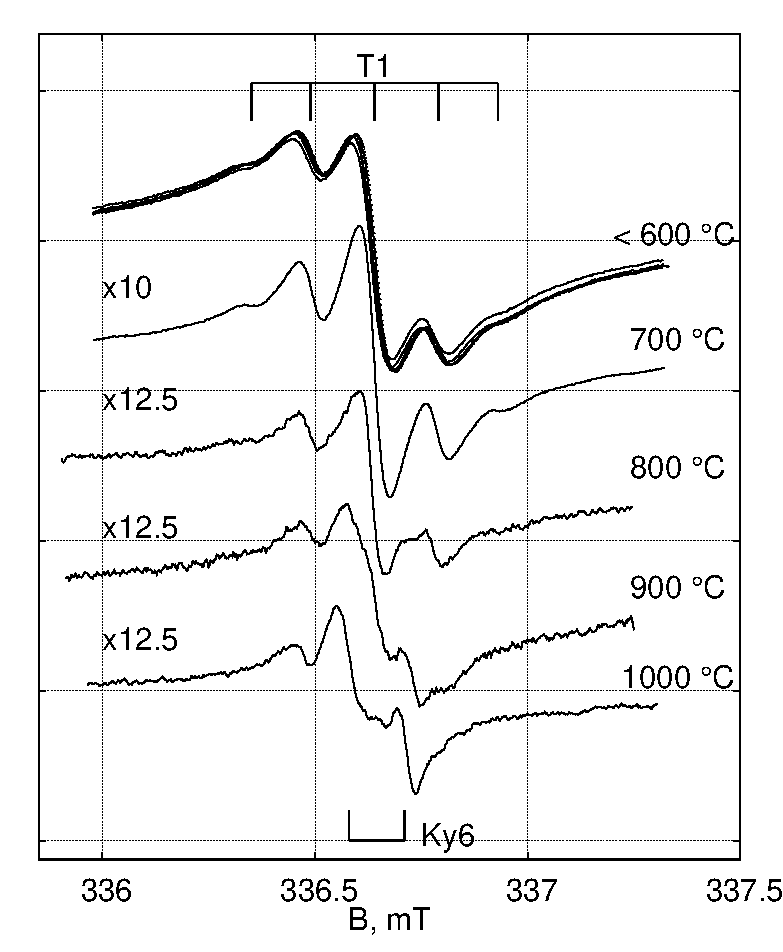
\includegraphics[width=200pt]{images/g1.eps}\mbox{}\\
figure 2\\
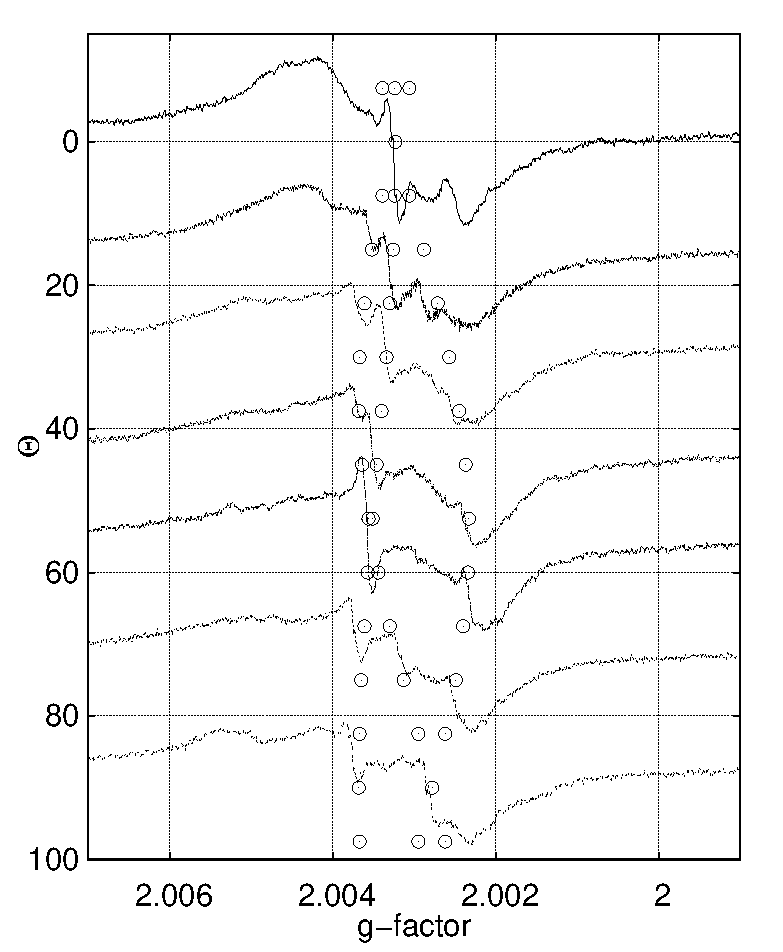
\includegraphics[width=200pt]{images/g2.eps}\mbox{}\\
figure 3\\
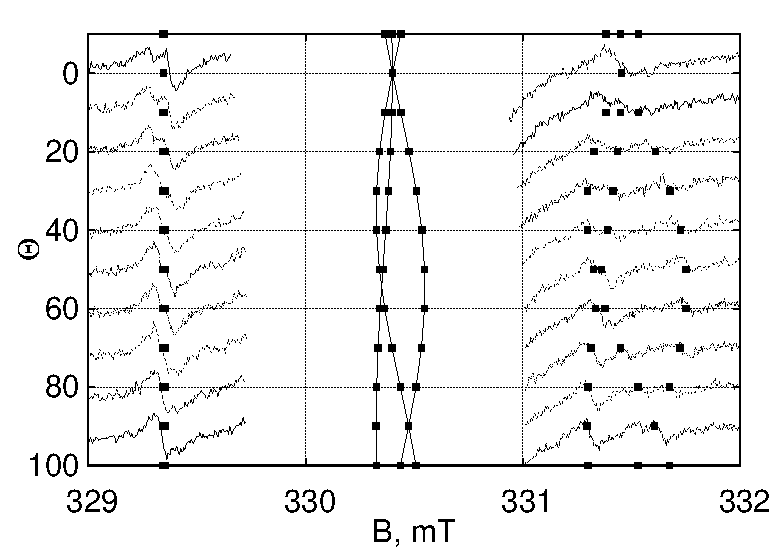
\includegraphics[width=200pt]{images/g3.eps}\mbox{}\\
figure 4\\
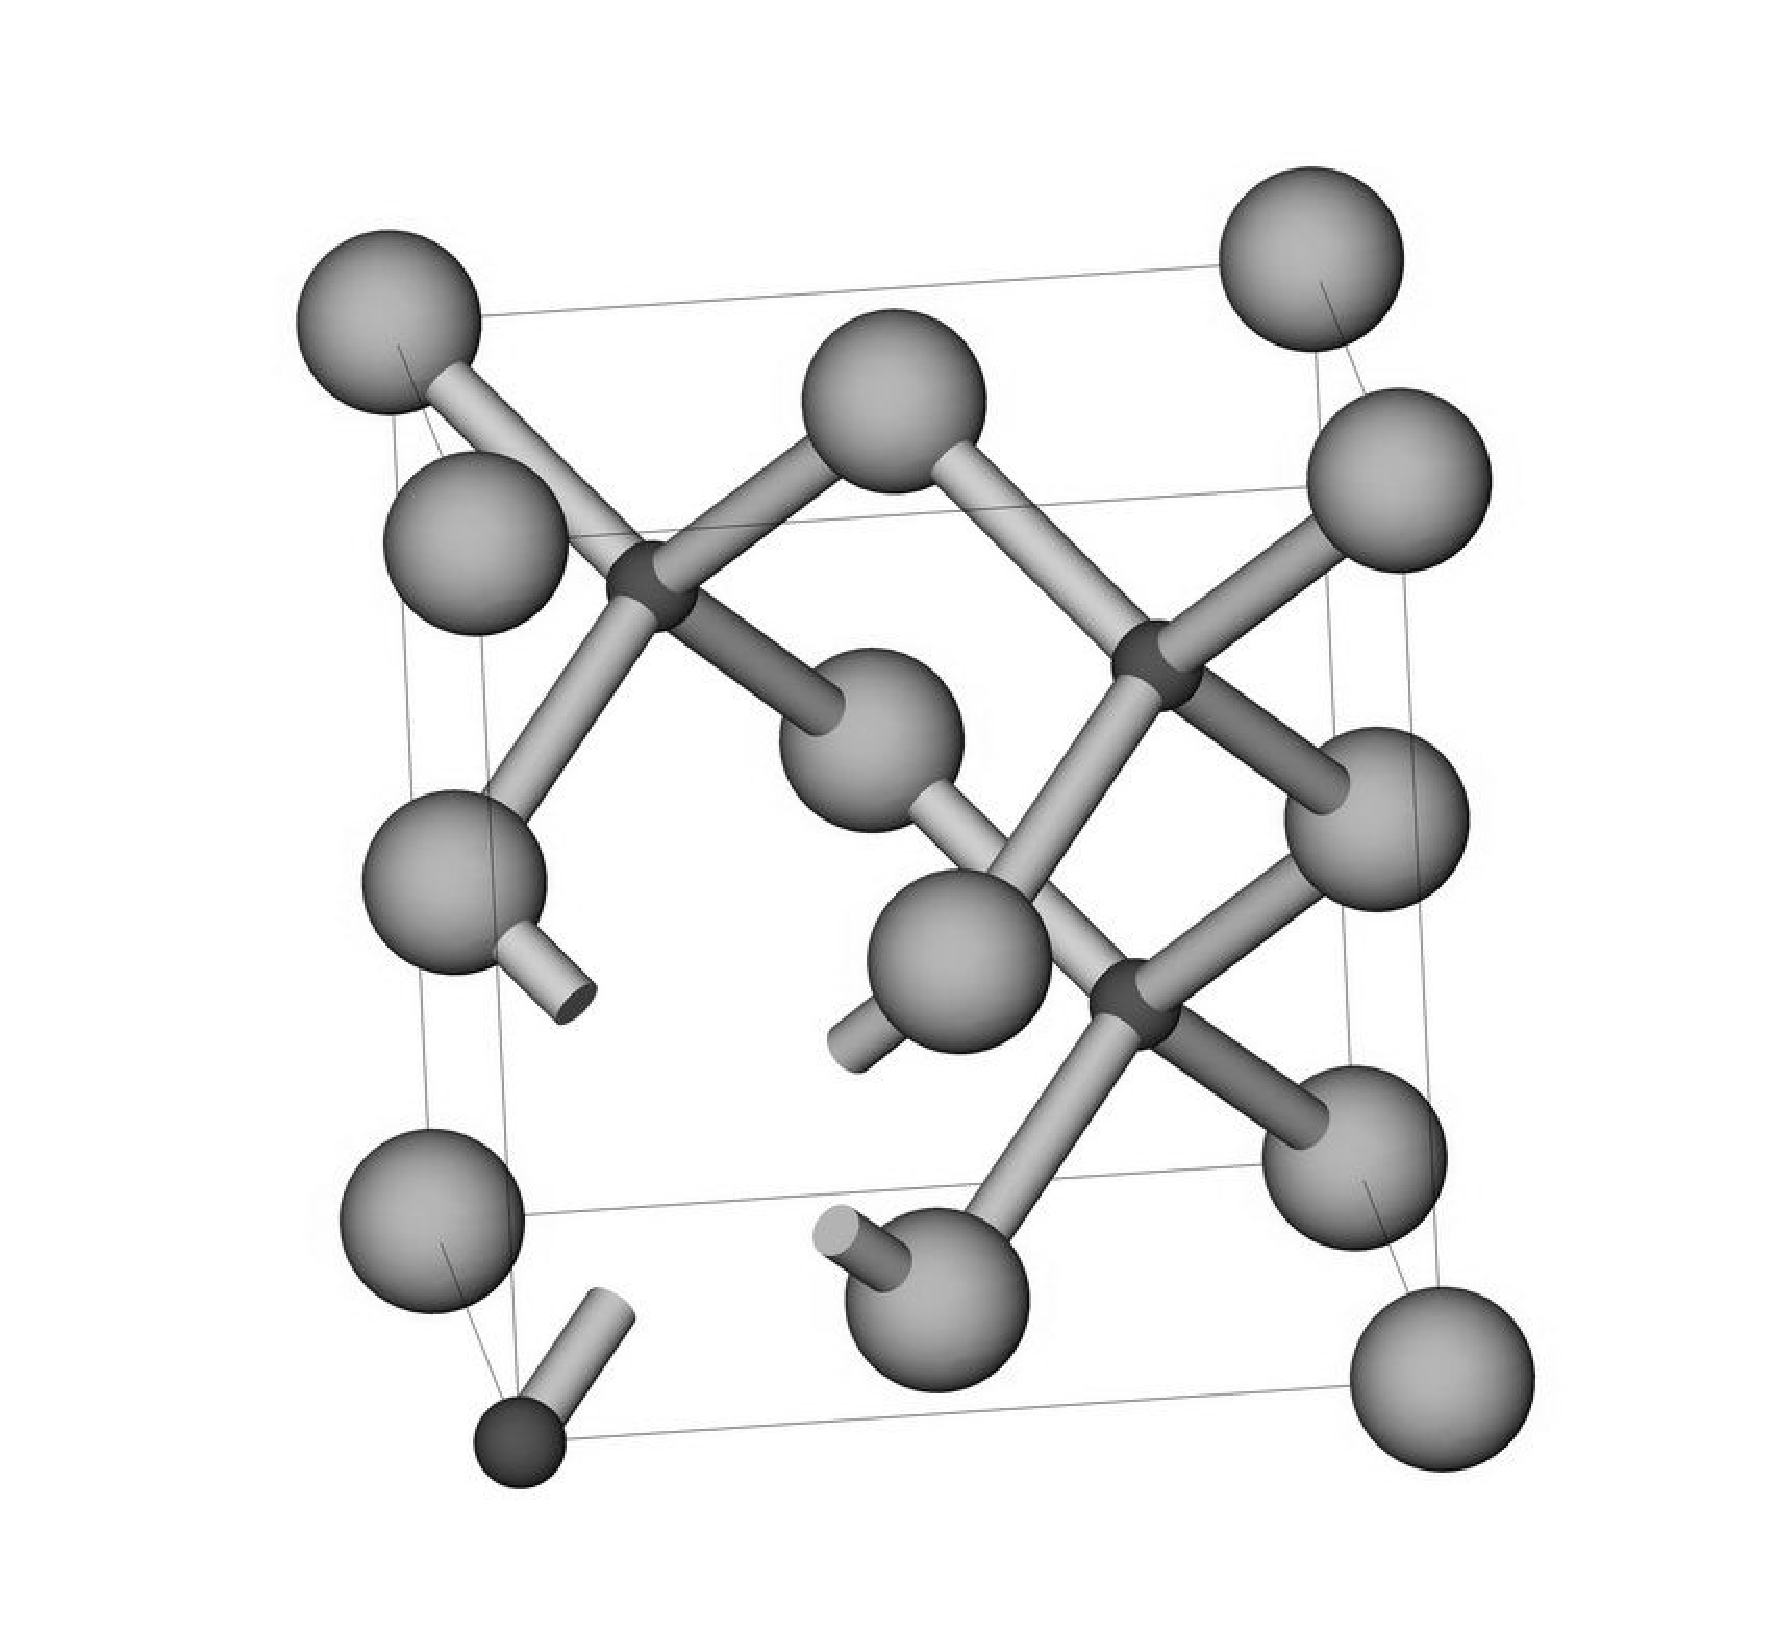
\includegraphics[width=200pt]{images/g4.eps}

\section{Conclusion}У даній роботі проведено дослідження кристалів 3C-SiC n-типу, опромінених реакторними нейтронами, спостережено та описано новий парамагнітний центр зі спіном S~=~1/2, названий Ку6. Аналіз його спектрів ЕПР, кінетики відпалу та поівняння отриманих результатів з теоретичними розрахунками потенційних бар'єрів та положень енергетичних рівнів, дають підґрунтя для побудови моделі даного дефекту та інтерпретувати його, як комплекс вакансія вуглецю - антисайт вуглецю у нейтральному зарядовому стані [V\textsubscript{C}C\textsubscript{Si}]\textsuperscript{0}.

%% \label{}

%% The Appendices part is started with the command \appendix;
%% appendix sections are then done as normal sections
%% \appendix

%% \section{}
%% \label{}

%% References
%%
%% Following citation commands can be used in the body text:
%%
%%  \citet{key}  ==>>  Jones et al. (1990)
%%  \citep{key}  ==>>  (Jones et al., 1990)
%%
%% Multiple citations as normal:
%% \citep{key1,key2}         ==>> (Jones et al., 1990; Smith, 1989)
%%                            or  (Jones et al., 1990, 1991)
%%                            or  (Jones et al., 1990a,b)
%% \cite{key} is the equivalent of \citet{key} in author-year mode
%%
%% Full author lists may be forced with \citet* or \citep*, e.g.
%%   \citep*{key}            ==>> (Jones, Baker, and Williams, 1990)
%%
%% Optional notes as:
%%   \citep[chap. 2]{key}    ==>> (Jones et al., 1990, chap. 2)
%%   \citep[e.g.,][]{key}    ==>> (e.g., Jones et al., 1990)
%%   \citep[see][pg. 34]{key}==>> (see Jones et al., 1990, pg. 34)
%%  (Note: in standard LaTeX, only one note is allowed, after the ref.
%%   Here, one note is like the standard, two make pre- and post-notes.)
%%
%%   \citealt{key}          ==>> Jones et al. 1990
%%   \citealt*{key}         ==>> Jones, Baker, and Williams 1990
%%   \citealp{key}          ==>> Jones et al., 1990
%%   \citealp*{key}         ==>> Jones, Baker, and Williams, 1990
%%
%% Additional citation possibilities
%%   \citeauthor{key}       ==>> Jones et al.
%%   \citeauthor*{key}      ==>> Jones, Baker, and Williams
%%   \citeyear{key}         ==>> 1990
%%   \citeyearpar{key}      ==>> (1990)
%%   \citetext{priv. comm.} ==>> (priv. comm.)
%%   \citenum{key}          ==>> 11 [non-superscripted]
%% Note: full author lists depends on whether the bib style supports them;
%%       if not, the abbreviated list is printed even when full requested.
%%
%% For names like della Robbia at the start of a sentence, use
%%   \Citet{dRob98}         ==>> Della Robbia (1998)
%%   \Citep{dRob98}         ==>> (Della Robbia, 1998)
%%   \Citeauthor{dRob98}    ==>> Della Robbia


%% References with bibTeX database:

%% \bibliographystyle{elsarticle-harv}
%% \bibliography{<your-bib-database>}

%% Authors are advised to submit their bibtex database files. They are
%% requested to list a bibtex style file in the manuscript if they do
%% not want to use elsarticle-harv.bst.

%% References without bibTeX database:

\begin{thebibliography}{50}

%% \bibitem must have one of the following forms:
        \bibitem{met1} A. Mattausch, M. Bockstedte, and O. Pankratov, Mater. Sci. Forum 353-356, (2001) 323.
    \bibitem{met2} M. Bockstedte, A. Mattausch, and O. Pankratov, Phys. Rev. B 68, (2003) 205201.
    \bibitem{brun1} F. Bruneval and G. Roma, Phys. Rev. B 83, 144116 (2011)
    \bibitem{choy1} W.J. Choyke, G. Pensl, MRS Bull. No. 3 (1997) 25
    \bibitem{hex1} J. Isoya, T. Umeda, N. Mizuochi, E. Janzen, T. Ohshima, Phys. Status Solidi B 245 (2008) 1298. 
    \bibitem{hex2} N.T. Son, B. Magnusson, Z. Zolnai, A. Ellison, E. Janzen, Mater. Sci. Forum 457-460 (2004) 437.
    \bibitem{epilay} W.J. Choyke, H. Matsunami, G. Pensl (Eds.), Silicon Carbide: Recent Major Advances, 2004, Springer, Berlin, Heidelberg.
    \bibitem{t1} H. Itoh, A. Kawasuso, T. Ohshima, M. Yoshikawa, I. Nashiyama, S. Tanigawa, S. Misawa, H. Okumura, S. Yoshida, Physica Status Solidi A 162 (1997) 173-198.
    \bibitem{ky5} V.Ya. Bratus’, R.S. Melnik, S.M. Okulov, V.N. Rodionov, B.D. Shanina, M.I. Smoliy, Physica B 404 (2009) 4739-4741.
    \bibitem{neut} F. Maekawa, K. Ochiai, K. Shibata, Y. Kasugai, M. Wada, Y. Morimoto, H. Takeuchi, Fusion Eng. Des. 58–59 (2001) 595.
    \bibitem{met3} E. Rauls, T. Lingner, Z. Hajnal, S. Greulich-Weber, T. Frauenheim, and J.-M. Spaeth, Phys. Status Solidi B 217 (2000), R1.
    \bibitem{met4} T. Lingner, S. Greulich-Weber, and J.-M. Spaeth, Mater. Sci. Forum 353-356, (2001) 505.

    %\bibitem{brun1} F. Bruneval and G. Roma, Phys. Rev. B 83, 144116 (2011)
%%   \bibitem[Jones et al.(1990)Jones, Baker, and Williams]{key}...
%%   \bibitem[Jones et al., 1990]{key}...
%%   \bibitem[\protect\citeauthoryear{Jones, Baker, and Williams}{Jones
%%       et al.}{1990}]{key}...
%%   \bibitem[\protect\citeauthoryear{Jones et al.}{1990}]{key}...
%%   \bibitem[\protect\astroncite{Jones et al.}{1990}]{key}...
%%   \bibitem[\protect\citename{Jones et al., }1990]{key}...
%%   \harvarditem[Jones et al.]{Jones, Baker, and Williams}{1990}{key}...
%%

% \bibitem[ ()]{}

\end{thebibliography}

\end{document}

%%
%% End of file `elsarticle-template-harv.tex'.
